\documentclass[11pt,compress,t,notes=noshow, aspectratio=169, xcolor=table]{beamer}

\usepackage{../../style/lmu-lecture}
% Defines macros and environments
% This file is included in slides and exercises

% Rarely used fontstyle for R packages, used only in 
% - forests/slides-forests-benchmark.tex
% - exercises/single-exercises/methods_l_1.Rnw
% - slides/cart/attic/slides_extra_trees.Rnw
\newcommand{\pkg}[1]{{\fontseries{b}\selectfont #1}}

% Spacing helpers, used often (mostly in exercises for \dlz)
\newcommand{\lz}{\vspace{0.5cm}} % vertical space (used often in slides)
\newcommand{\dlz}{\vspace{1cm}}  % double vertical space (used often in exercises, never in slides)
\newcommand{\oneliner}[1] % Oneliner for important statements, used e.g. in iml, algods
{\begin{block}{}\begin{center}\begin{Large}#1\end{Large}\end{center}\end{block}}

% Don't know if this is used or needed, remove?
% textcolor that works in mathmode
% https://tex.stackexchange.com/a/261480
% Used e.g. in forests/slides-forests-bagging.tex
% [...] \textcolor{blue}{\tfrac{1}{M}\sum^M_{m} [...]
% \makeatletter
% \renewcommand*{\@textcolor}[3]{%
%   \protect\leavevmode
%   \begingroup
%     \color#1{#2}#3%
%   \endgroup
% }
% \makeatother


\title{Interpretable Machine Learning}
% \author{LMU}
%\institute{\href{https://compstat-lmu.github.io/lecture_iml/}{compstat-lmu.github.io/lecture\_iml}}
\date{}

\begin{document}

\newcommand{\titlefigure}{figure/h-statistic}
\newcommand{\learninggoals}{
\item Understand the Friedman's H-statistic
\item How to measure the overall interaction strength
\item How to measure 2-way interaction strengths
%\item Understand how to interpret ICE curves and PD plots
}

\lecturechapter{Friedman's H-Statistic}
\lecture{Interpretable Machine Learning}

\begin{vbframe}{Pre-thoughts}
	
		\textbf{Idea}: If two features do not interact, we can decompose the PD function (assuming it is centered at zero) by:
	

	$$\fh_{jk, PD}(x_j, x_k) = \fh_{j, PD}(x_j) + \fh_{k, PD}(x_k)$$

\begin{itemize}
	\item $\fh_{jk, PD}(x_j, x_k)$ is the 2-dim PD function of both features $j$ and $k$.
	\item $\fh_{j, PD}(x_j)$ and $\fh_{k, PD}(x_k)$ are the PD functions of the single features.
\end{itemize}

	Similarly, if a feature does not interact with any other feature, we can decompose the prediction function by:

	$$\fh(x) = \fh_{j, PD}(x_j) +  \fh_{-j, PD}(x_{-j}).$$

\begin{itemize}
	\item $\fh(x)$ is the prediction function of the considered model.
	\item $\fh_{j, PD}(x_j)$ is the PD function of feature $j$.
	\item $\fh_{-j, PD}(x_{-j})$ is the PD function of all features except feature $j$.
\end{itemize}
\end{vbframe}

\begin{vbframe}{Example \& Problem}
Imagine the following (fictive) data situation:
\begin{table}[ht]
\centering
\begin{tabular}{rllr}
  \hline
 workingday & weather & count \\ 
  \hline
    NO & MISTY & 1000 \\ 
    YES & GOOD & 1349 \\ 
    YES & MISTY & 1510 \\ 
    NO & GOOD & 822 \\ 
   \hline
\end{tabular}
\end{table}
\begin{itemize}
    \item Constant $\fh_(x_{workingday} = "YES", x_{weather} = "GOOD") = 1349$ (it the PD is centered this term can be ignored
    \item Partial Dependence on Workingday: $\fh_{workingday, PD}(x_{workingday} = "NO") = -527$
    \item Partial Dependence on Weather: $\fh_{weather, PD}(x_{weather} = "MISTY") = 161$
    \item<2> If there was no Feature Interaction: $\fh_(x_{workingday} = "NO", x_{weather} = "MISTY") = 1349 -527 +161 =983$
    \item<2> The constant of 17 is the remaining interaction of the two features $u_{workingday, weather}$, given that there is no error.
\end{itemize}


\end{vbframe}

\begin{vbframe}{Problem \& Idea}
    
    \textbf{Problem}:
	Often, when features interact with each other in a prediction model, the \textbf{prediction cannot be expressed as the sum of the feature effects}, because the effect of one feature depends on the value of the other feature. ´
    \vspace{1cm}
    
    \textbf{Idea}:
       Decompose the prediction into three terms: 
   \begin{itemize}
       \item a term for the first feature
       \item a term for the second feature
       \item \textbf{a term for the interaction between the two features}
   \end{itemize}
    

    \begin{eqnarray}
    \fh_{jk, PD}(x_j, x_k) &=& \fh_{j, PD}(x_j) + \fh_{k, PD}(x_k) + u_{jk} \\
    u_{jk} &=& \fh_{jk, PD}(x_j, x_k) - \fh_{j, PD}(x_j) + \fh_{k, PD}(x_k)  
    \end{eqnarray}
    
    \textbf{Note:} This Idea ca also be generalized to mutltiple features.
	
\end{vbframe}


\begin{vbframe}{2-way Interaction Strength}
Based on this idea, the H-statistic proposed by Friedman and Popescu measures the interaction strength between feature $j$ and $k$ by:

	$$H^2_{jk} = \frac{\sum_{i=1}^n\left[\fh_{jk,PD}(x_j^{(i)}, x_k^{(i)}) - \fh_{j, PD}(x_j^{(i)}) - \fh_{k, PD}(x_k^{(i)})  \right]^2}{\sum_{i=1}^n \left[\fh_{jk,PD}(x_j^{(i)}, x_k^{(i)}) \right]^2}$$

\textbf{Note}: The numerator is $0$ if the two features $x_j$ and $x_k$ do not interact, i.e., $\fh_{jk, PD}(x_j, x_k) - \fh_{j, PD}(x_j) - \fh_{k, PD}(x_k) = 0$.

$\Rightarrow$ The smaller the values of $H^2_{jk}$, the weaker the interaction between $x_j$ and $x_k$.


\footnote[frame]{Friedman, Jerome H., and Bogdan E. Popescu (2008). Predictive learning via rule ensembles. The Annals of Applied Statistics. JSTOR, 916–54.}

\end{vbframe}


\begin{vbframe}{Overall Interaction Strength}

Similarly, it is possible to measure whether a feature $j$ interacts with any other feature (Overall interaction strength):

\begin{onlyenv}<1>
$$H^2_{j} = \frac{\sum_{i=1}^n\left[u^{(i)}_{j,k} \right]^2}{\sum_{i=1}^n \left[\fh(x^{(i)}) \right]^2}$$
\end{onlyenv}
\begin{onlyenv}<2>$$H^2_{j} = \frac{\sum_{i=1}^n\left[\fh(x^{(i)}) - \fh_{j, PD}(x_j^{(i)}) - \fh_{-j, PD}(x_{-j}^{(i)})  \right]^2}{\sum_{i=1}^n \left[\fh(x^{(i)}) \right]^2}$$
\end{onlyenv}
\textbf{Example}: Inspect interactions of a random forest for the bike data

\begin{center}
	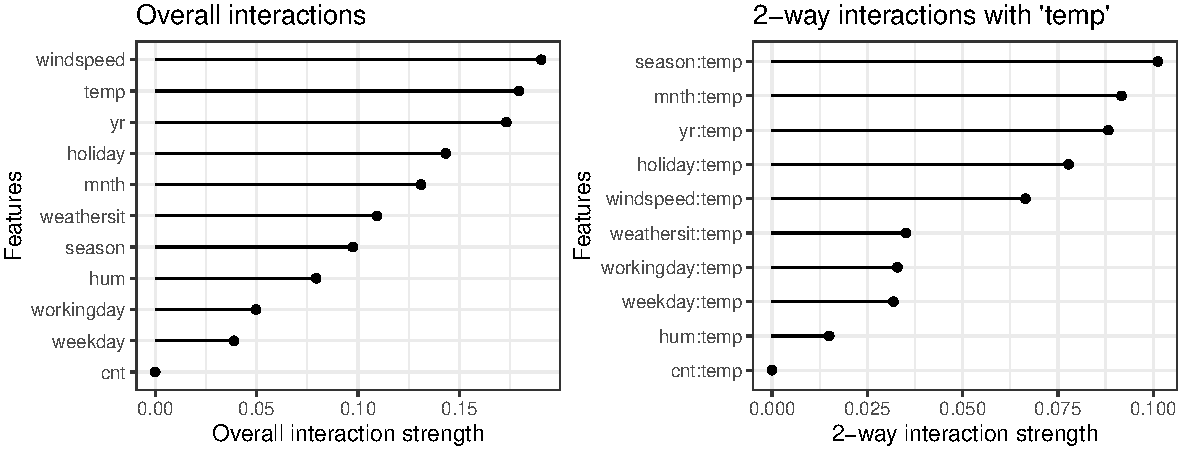
\includegraphics[width=0.7\textwidth]{figure/h-statistic}
\end{center}
\end{vbframe}


\begin{vbframe} {unnormalized H}
\begin{itemize}
    \item When the total effect of two features is weak, but mostly consists of interactions, than the H-statistic will be very large.
    \item These spurious interactions spurious interaction can be easily overinterpreted as a strong interaction effect, when in reality both features play a minor role in the model.
    \item A possible remedy is to visualize the \textbf{unnormalized version of the H-statistic}
\end{itemize}

$$
H_{j k}^{*}=\sqrt{\sum_{i=1}^{n}\left[P D_{j k}\left(x_{j}^{(i)}, x_{k}^{(i)}\right)-P D_{j}\left(x_{j}^{(i)}\right)-P D_{k}\left(x_{k}^{(i)}\right)\right]^{2}}
$$

$\Rightarrow$ This scales the H-statistic to the same level as the response and puts less emphasis on spurious interactions.
\end{vbframe}

\begin{vbframe}{Discussion}
\textbf{Advantages}
\begin{itemize}
    \item Underlying theory: the partial dependence decomposition.
    \item Meaningful interpretation: The interaction is defined as the share of variance that is explained by the interaction.
    \item Since the statistic is dimensionless, it is comparable across features and even across models.
    \item Detects all kinds of interactions, regardless of their particular form.
    \item Possibility to analyze arbitrary higher interactions such as the interaction strength between 3 or more features.
\end{itemize}

\textbf{Disadvantages}
\begin{itemize}
    \item Computation involves estimating marginal distributions. These estimates also have a certain variance if we do not use all data points. This means that as we sample points, the estimates also vary from run to run and the results can be unstable.
    \item Yet, there is no statistical test available in a model-agnostic version.
    \item No information about the "shape" of interactions. That is what partial dependence plots are for.
    \item If the features correlate strongly we integrate over feature combinations that are very unlikely in reality.
\end{itemize}

	

\end{vbframe}

\endlecture
\end{document}

